\documentclass[titlepage,oneside,a4paper,10pt]{article}%openright,
\usepackage{a4,graphicx,fancyhdr}
\usepackage[english]{babel} 
\usepackage{natbib}
\usepackage[utf8]{inputenc}
\usepackage[bf,footnotesize]{caption}
\usepackage{hyperref}
\usepackage[percent]{overpic}
\usepackage{color}
\usepackage{makeidx}
\usepackage[bottom]{footmisc}
\usepackage{amsmath,amssymb}
\usepackage{subcaption}
\usepackage[rightcaption]{sidecap}
\usepackage{placeins}
\usepackage{float}
\usepackage{listings}
\usepackage{booktabs} % nice tabulars
\usepackage{siunitx} % for proper writing of numbers with units
\usepackage{todonotes} % make notes in latex document

%\input amssym.def
%\input amssym.tex

\setlength{\hoffset}{-1in}%
\setlength{\oddsidemargin}{2cm}%
\setlength{\evensidemargin}{3cm}%
\setlength{\textwidth}{16cm}%
\setlength{\headheight}{15pt}%


\parindent 0pt											%Einzug nach eine Absatz mit \par

\pagestyle{fancy}%
\renewcommand{\sectionmark}[1]{\markright{\thesection\ #1}}%
\lhead[\thepage]{\rightmark}%
\rhead[\leftmark]{\thepage}%
\cfoot{}%

\definecolor{middlegray}{rgb}{0.5,0.5,0.5}

\lstset{language=C++,
                basicstyle=\ttfamily,
                keywordstyle=\color{blue}\ttfamily,
                stringstyle=\color{red}\ttfamily,
                commentstyle=\color{middlegray}\ttfamily,
                morecomment=[l][\color{magenta}]{\#}
}

\bibliographystyle{apalike}

\begin{document}
    \begin{titlepage}
\makebox[0.9\paperwidth][r]{
\includegraphics[height=1.3cm]{UiO_A_ENG.pdf}}\\

    \vspace{3.5cm}
    \center
    {\hspace{5mm}\Large\bf Computational Physics: Project 3}\\
    \vspace{1.5cm}
    {\hspace{5mm}\huge\textbf{Variational Monte Carlo project}}\\
    \vspace{4cm}
    {\hspace{5mm}\Large\bf Jannes Klee}\\
    \vspace{1cm}
    {\hspace{5mm}\Large\bf Anja Bielefeld}\\
    \vspace{1.5cm}
    {\hspace{5mm}\large \today}\\
    \vspace{1.5cm}
\end{titlepage}
\pagenumbering{gobble}
\tableofcontents

    \pagenumbering{arabic}
    \section{Introduction}



In this report we will be using natural units:
\begin{align*}
\hbar = c = e = m_e = 1\\
\Rightarrow [E] = \mathrm{a.u.},
\end{align*}
where $\hbar$ is the Planck constants divided by $2\pi$, $c$ is the speed of light, $e$ is the elemantary charge and $m_e$ is the electron mass. The unit of enegry than becomes atomic units, denoted as a.u.
	\section{The physical problem}\label{sec:problem}
Quantum dots are nanoscopic crystals usually from semiconducting materials being of a size to exhibit quantum mechanical properties. In this report we will look at systems of electrons confined in a harmonic oscillator, which acts like a trap. These systems can be considered quantum dots. In order to study any system like that, we have to look at the Hamiltonian, which consists of two parts:
\begin{equation}
\hat{H} = \hat{H_0} + \hat{H_1},
\end{equation}
where $\hat{H_0}$ describes the standard harmonic oscillator and $\hat{H_1}$ the repulsive term between the charged particles (in this case electrons). We can than write
\begin{equation}
\hat{H} = \sum_{i=1}^N \left( -\frac{1}{2} \nabla_i^2 + \frac{1}{2} \omega^2 r_i^2 \right) + \sum_{i<j} \frac{1}{r_{ij}}
\end{equation}
The quantity $N$ denotes the number of charged particles, $\omega$ is the oscillator frequency, $r_i$ is the position of particle $i$ given by $r_i = \sqrt{r_{ix}^2 + r_{iy}^2}$ and distance between two particles is referred to as $r_{ij} = \sqrt{\mathbf{r_1}- \mathbf{r_2}}$.\\
From quantum mechanics we know, that the wave function corresponding to this Hamiltonian for one electron in two dimensions $(x,y)$ is
\begin{equation}\label{glg:wavefunc1}
\phi_{n_x,n_y}(x,y) = A H_{n_x} (\sqrt{\omega} x) H_{n_y} (\sqrt{\omega} y) \exp\left[-\frac{\omega}{2} (x^2+y^2)\right].
\end{equation}
In this equation the Hermite polynomials $H_{n_x} (\sqrt{\omega} x)$ appear as well as the constant $A$, which is there because of the normalization.\\
To get the energy $E$, we have to consider the Eigenvalue equation
\begin{equation}\label{glg:eigenvalue}
\hat{H} \phi_\lambda = E \phi_\lambda,
\end{equation}
which leads to the energy
\begin{equation}
E_{n_x,n_y} = \omega(n_x + n_y +1)
\end{equation}
Looking at the lowest energy state we have $E_{(1)}=\omega$.\\
Advancing now to the case of two electrons who do not repell each other we have two independent Hamiltonians, one for each electron, and as a result two independent eigenvalue problems as in euqation~\ref{glg:eigenvalue}. This leads to the same energy as before, but this time the energy must be taken into account twice. So we get:
\begin{equation}
E_{(2)} = E_{(1)} + E_{(1)} = 2 E_{(1)}.
\end{equation}
The corresponding wave function is then given by
\begin{equation}
\Phi(\mathbf{r_1},\mathbf{r_2}) = C \exp\left[-\frac{\omega}{2} (r_1^2+r_2^2)\right].
\end{equation}
As in equation~\ref{glg:wavefunc1} $C$ is the normalization constant.\\
Since the particles we are considering are fermions, we must regard the spin as well. The overall spin must be zero, because according to the Pauli principle two fermions cannot have the same quantum numbers. The electrons we are looking at are having exactly the same energy of $E = \omega$, so their only way of obeying the princple is to have different spins. There are two possible states:
\begin{equation}
|\uparrow \downarrow > \text{~and~} |\downarrow \uparrow >
\end{equation}
Hence one of the electrons has spin 1/2 and the other one has spin -1/2. Despite this they are indistinguishable, so both states are possible.\\
Regarding the wave function there we will now make an Ansatz for simplifying the wave function $\psi$:
\begin{align}
\psi (\mathbf{r_1,\sigma_1,r_2, \sigma_2}) = R(\mathbf{r_1,r_2}) X (\mathbf{\sigma_1, \sigma_2})
\intertext{with}
R(\mathbf{r_1,r_2}) = \varphi_{n_{x_1} n_{y_1}}(x_1, y_1) \varphi_{n_{x_2} n_{y_2}}(x_2, y_2)
\end{align}
In this Ansatz $R(\mathbf{r_1,r_2})$ is the part of the wave function depending on the positions and $X (\mathbf{\sigma_1, \sigma_2})$ is the spin-depending part, the matrices $\mathbf{\sigma_1}$ and $\mathbf{\sigma_2}$ are the spin matrices for particle 1 and 2.\\
According to this Ansatz we can focus on the position-based part of the wave function for the following analysis.

    \section{The method}\label{sec:algo}
As presented in the previous section the eigenvalue problem of two electrons in a harmonic oscillator without any interaction terms can be easily solved. Looking at electrons in a quantum dot this calculation gains complexity. This is why we introduce the Variational Monte Carlo Method for estimating the electron states.
\subsection{Variational Monte Carlo method}
In the Variational principle, we take the eigenvalue problem from equation~\ref{glg:eigenvalue} and expand the wave function as following:
\begin{equation}
\varphi_0 = \sum_{\lambda=0}^{\infty} c_{0 \lambda} \psi_{\lambda},
\end{equation}
where $c_{0 \lambda}$ are coefficients.\\
In quantum mechanics the energy is the expectation value
\begin{align}
E = &\frac{\langle \psi_0 | \hat{H} | \psi_0 \rangle}{\langle \psi_0 | \psi_0 \rangle}\\
\intertext{So when we apply the expansion to this, we get:}
&\frac{\langle \varphi_0 | \hat{H} | \varphi_0 \rangle}{\langle \varphi_0 | \varphi_0 \rangle}\\
= &\frac{\sum_{\alpha,\beta}c_{0\alpha}^*c_{0 \beta} \int d\tau \psi_{\alpha}^*(\tau)\hat{H}\psi_{\beta}(\tau)}{\sum_{\alpha,\beta}c_{0\alpha}^*c_{0 \beta} \int d\tau \psi_{\alpha}^*(\tau)\psi_{\beta}(\tau)}\\
= &\frac{\sum_{\alpha} E_{\alpha} |c_{0\alpha}|^2}{\sum_{\alpha} |c_{0\alpha}|^2},
\end{align}
because by construction $\langle\psi_{\alpha}| \psi_{\beta}\rangle = \delta_{\alpha \beta}$ for eigenfunctions $\psi_{\alpha},\psi_{\beta}$.\\
We have to consider two cases now:
\begin{itemize}
\item If the expansion $\varphi_0$ is not the eigenfunction $\psi_0$ we get the an energy
\begin{equation}
E_0 \leqslant \frac{\langle \varphi_0 | \hat{H} | \varphi_0 \rangle}{\langle \varphi_0 | \varphi_0 \rangle}.
\end{equation}
\item If the expansion $\varphi_0$ corresponds exactly to the eigenfunction $\psi_0$ we get the exact energy
\begin{equation}
E_0 = \frac{\langle \varphi_0 | \hat{H} | \varphi_0 \rangle}{\langle \varphi_0 | \varphi_0 \rangle}.
\end{equation}
\end{itemize}
In the second case the variance of the energy
\begin{equation}
\mathrm{var}(E) = \langle H^2 \rangle - \langle H\rangle^2 = 0.
\end{equation}
As the expansion wave function $\varphi_0$ we use a trial wave function we will call $\psi_T (\mathbf{r_1, r_2},\alpha, /beta)$, with $\alpha$ and $\beta$ being the variational parameters. In this report the trial wave function for two electrons has the form:
\begin{equation}\label{eq:trialwavefunction}
\psi_T(\mathbf{r_1,r_2}) = C \exp\left[-\alpha\frac{\omega}{2} (r_1^2+r_2^2)\right] \exp \left[ \frac{a_{12} r_{12}}{(1+\beta r_{12})} \right]
\end{equation}
with
\begin{align}
a_{12} =\left\{\begin{array}{cl} 1, & \mbox{for} \uparrow\downarrow\\ 1/3, & \mbox{for} \uparrow\uparrow,\downarrow\downarrow \end{array}\right]
\end{align}
and
\begin{equation}
r_{12} = \sqrt{\mathbf{r_1} - \mathbf{r_2}}.
\end{equation}
The factor $J = \exp \left[ \frac{a_{12} r_{12}}{(1+\beta r_{12})} \right]$ is called the Jastrow factor, which we will refer to later.\\
In order to find the wave function and its corresponding energy to the case we are considering, we compute the expectation value $E(\alpha, \beta)$ and find its minimum or alternatively the minimum of its variance $\mathrm{var}(E(\alpha, \beta))$. This procedure is used in section~\ref{sec:result}. For the six electron case, the variational wave function becomes as in equation~\ref{glg:6electron} and we can again search the minimum energy.\\
%Slater determinant -> six electron stuff
\subsection{Monte Carlo methods}
The basis of the method explained above are the Monte Carlo methods, which can be referred to as statistical simulation methods. The central building block of these methods is the propability distribution function (PDF), which is used to describe and characterize the physical problem. This does not restrict the method to statistical problems, but by displaying the desired solution in terms of PDF's, non-stochastic problems can be handled as well. During a Monte-Carlo simulation, random numbers must be generated covering an interval uniformly. Using these numbers, many random samples are taken from the PDF. In order to get the desired result the average of all samples is computed. According to this, the precision of the simulation rises with the amount of samples. The error has to be estimated to get an impression of the simulation's precision.\\
On the contrary of statistical random number-based methods, in standard mathematical modelling, the problem would be distretized and solved by a numerical approach.\\
\subsubsection{Pseudo-random number generation}\label{sec:ran}
As a main ingredient, random numbers play as important role in Monte-Carlo simulations and therefore have to be 'as random as possible'. The generation of truely random numbers is practically not possible, this is why the random numbers we work with are pseudo-random, generated by an algorithm fullfilling the criteria of
\begin{itemize}
\item generating equally distributed numbers in a given interval (usually [0,1])
\item repeating random number sequences seldom
\item being fast
\item generating insignificantly correlated numbers
\end{itemize}
I this report, we use random number generators explained in~\cite{numerical}, that are called \texttt{ran0} and \texttt{ran1}.\\
Furthermore, we generate random gaussian distributed random numbers using \texttt{gaussian}. 
% Jetzt nutzen wir andere 
\subsection{Metropolis algorithm}\label{sec:metropolis}
The difficult part of Monte-Carlo simulations is the selection rule for random states. One must find a method when to reject and when to accept the generated state. Precision and efficiency strongly depend on this rule. Supposing we have a distribution such as the one shown in figure~\ref{fig:distribution} and we have already picked an initial random variable at $r_i$. Since we are performing the simulation on many samples, we now have to pick a new random number keeping in mind, that there are two cases, which must be avoided:
\begin{itemize}
\item Choosing repeatedly numbers very close to the initial value such as $r_j$ in figure~\ref{fig:distribution}. We would then 'get stuck' around the interval of $r_i$ and therefore loose the overview of the function we are evalutating.
\item Jumping to numbers far away from the initial value, where the distribution is negligable, for example to $r_k$ in figure~\ref{fig:distribution}. 
\end{itemize}
\begin{figure}[htbp]
    \centering
    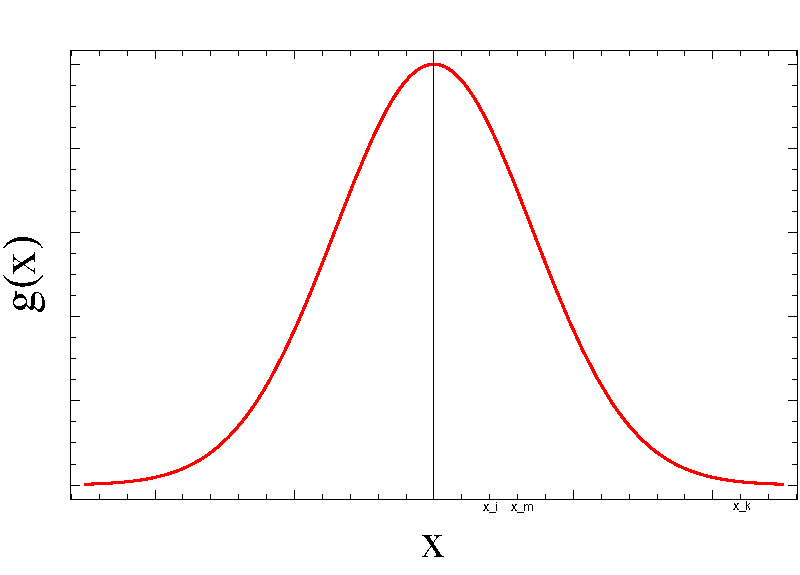
\includegraphics[scale=0.45]{distribution}
    \caption{Gaussian distribution showing problems in selection of random states}
    \label{fig:distribution}
\end{figure}
Preventing the simulation in creating biased averages and unprecise results is possible by using the Metropolis algorithm, which is a Markov process, satisfying both ergodicity and detailed balance.\\
Ergocidity in random processes means, that the time average of a sequence of events has to be the same as the average of all possible states, the so-called ensemble-average. In order to obey detailed balance, the process must follow a distribution, where the transition propability from state $i$ to state $j$ is the same as from state $j$ to state $i$ at equilibrium. This is also called reversibility.\\
Markov chains are referred to as random walks with selected propability to make a move, which is independent of the previous step. An example of this movement is the Brownian random walk shown in figure~\ref{fig:Brown}, where a particle moves in the $x$-$y$-plane with step length 1 preforming hundred steps. The propability of moving is the same for every direction. Using Markov processes, we can generate new random states and reach the most likely state (equilibrium) after a certain time.
%ergodicity
%detailed balance
\begin{figure}[htbp]
    \centering
    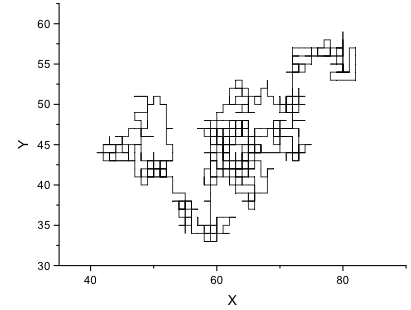
\includegraphics[scale=0.6]{Brown}
    \caption{Brownian random walk of 100 steps in $x$-$y$-plane and step length 1}
    \label{fig:Brown}
\end{figure}
\FloatBarrier
\subsubsection{Importance sampling}\label{sec:importance}
There are lots of examples in science, where biasing is disturbing and should be avoided. One example are the required unbiased uncorrelated random numbers in section~\ref{sec:ran}. In Monte-carlo methods, biasing can be a tool to increase the simulation's efficiency by preforming a Metropolis walk biased by the trial wave function. Since our problem is somewhat simular to a diffusion process in one dimension for one particle, we may use an approach based on the Fokker-Planck and the Langevin equation.\\
The 'old' and 'new' positions in space can be caluclated by
\begin{align}
r_{old} &= \eta\\
r_{new} &= r_{old} + \eta + \delta t D F_{old},
\end{align}
where $\eta$ denotes a gaussian distributed random variable, $\delta t$ refers to the time step, $D$ is the diffusion constant, which is in our case set to $D=0.5$ and $F_{old}$ is the quantum force at position $r_{old}$. Note, that $\eta$ are different random numbers.\\
The term responsible for biasing the walk in space $x$ is the quantum force, which leads the walk to regions with large trial wave function. In a brute force Metropolis algorithm, the propability of moving would be the same for all directions. The quantum force is
\begin{equation}\label{eq:quantum_force}
\mathbf{F} = 2 \frac{1}{\psi_T} \mathbf{\nabla} \psi_T
\end{equation}
In order to include this biasing in the Metropolis algorithm, we will replace
\begin{align}
q(r_{old},r_{new}) &= \frac{\vert \psi_T(r_{new})\vert^2}{\vert \psi_T(r_{old})\vert ^2}
\intertext{by}
q(r_{old},r_{new}) &= \frac{G(r_{old},r_{new},\delta t) \vert \psi_T(r_{new})\vert^2}{G(r_{new},r_{old},\delta t) \vert \psi_T(r_{old})\vert^2},
\intertext{where the quantity $G$ refers to the Greensfunction}
G(y,x,\delta t) &= \frac{1}{(4\pi D\delta t)^{3N/2}} \exp\left[-(y-x-D \delta t F(x))^2 \frac{1}{4D \delta t} \right]
\end{align}


\subsection{Closed form solutions}
The quantum force (eq. \ref{eq:quantum_force}) and the kinetic energy part \todo{referenzierung auf funktion} are till now calculated with a brute force derivation. A disadvantage of this method is that the wavefunction has to be evaluated multiple times at different positions $r+h$, $r-h$ respectively. In order to optimize this step one can implement the analytical expressions. These are derived in \citet{hogberget2013}. The quantum force can thereby be expressed by
\begin{equation}
\mathbf{F_i} = 2 \left( \frac{\nabla_i |\mathbf{S\uparrow}|}{|\mathbf{S\uparrow}|} + \frac{\nabla_i J}{J} \right).
\end{equation}
The first part of the right side denotes the gradient of the Slater determinant, the second one the gradient of the Jastrow factor. It has to be payed attention that this is the expression for only one particle with index $i$ moved with spin up. Considering a spin down particle the $|\mathbf{S\uparrow}|$ becomes $|\mathbf{S\downarrow}|$. Further the kinetic part of the local energy arises as a result of
\begin{equation}
\frac{\nabla_i^2 \Psi_T}{\Psi_T} = \frac{\nabla_i^2 |\mathbf{S\uparrow}|}{|\mathbf{S\uparrow}|} + \frac{\nabla_i^2 J}{J} + 2\left( \frac{\nabla_i |\mathbf{S\uparrow}|}{|\mathbf{S\uparrow}|} \cdot \frac{\nabla_i J}{J} \right),
\end{equation}
again assuming a spin up particle.

The missing expressions can be obtained by deriving the trial wavefunction \ref{glg:6electron}. This is also done in \citet{hogberget2013} and reveals 
\begin{equation}\label{eq:jastrow-derivations}
    \frac{\nabla_i J}{J} = \sum_{k\neq i = 1}^{N}\frac{a_{ik}}{r_{ik}} \frac{\mathbf{r_i}-\mathbf{r_k}}{\left(1 + \beta r_{ik} \right)^2}
\end{equation}
for the gradient and 
\begin{equation}
    \frac{\nabla_i^2 J}{J} = \left| \frac{\nabla_i J}{J} \right| - \sum_{k\neq i = 1}^{N}a_{ik} \frac{\beta r_{ik} - 1}{r_{ik}\left(1 +\beta r_{ik} \right)^3} 
\end{equation}
for the laplacian of the jastrow factor. The variables and constants are the already known ones of equation \ref{} \todo{referenz zu trialwavefunction für viele teilchen}. The derivations of the Slater determinants can be calculated to
\begin{equation}\label{eq:gradientslater}
    \frac{\nabla_i |\mathbf{S}|}{|\mathbf{S}|} = \sum_k \left( \nabla_i \phi_k(\mathbf{r}_i)\right)(\mathbf{S}_{ki}^{-1})
\end{equation}
for the gradient and
\begin{equation}\label{eq:laplacianslater}
    \frac{\nabla_i^2 |\mathbf{S}|}{|\mathbf{S}|} = \sum_k^{N/2} \left( \nabla_i^2 \phi_k(\mathbf{r}_i)\right)(\mathbf{S}_{ki}^{-1})
\end{equation}
for the laplacian. For the first part on the right side of eqs. \ref{eq:gradientslater} and \ref{eq:laplacianslater} exists analytical expressions which can be determined by applying the operands on the single particle equation \ref{glg:wavefunc1}. These can also be found in tabulated form in \citet[app. D]{hogberget2013}. The last term $\mathbf{S}_{ki}^{-1}$ is the transpose of the inverse Slater matrix. 

The closed form solutions are fully implemented in the code and can be found at Github on the branch \texttt{closed\_form}. Unfortunately there were still unresolved problems which yielded to non-correct energies in the solutions (details in the evaluation). 

	\section{Results and discussion}\label{sec:result}
We will now first take a look at the case of two electrons in a potential with different oscillator energies. In order to do so, we perform a Variational Monte Carlo simulation and use the Metropolis algorithm explained in section~\ref{sec:metropolis} to find the energy of the ground state. Therefor we use numerical derivation. We will later introduce analytical calculations based on closed-form expressions as well (section~\ref{sec:analytical}). Besides, we put emphasis on the correlations introduced by the Jastrow factor by computing the kinetic and potential energy of the ground state for different oscillator frequencies.\\
In addition we introduce importance sampling and analyse the dependency of the results to the time step $\delta t$.\\
\subsection{Two electron case}\label{sec:2electron}
Since it is the easiest case, we first look at two electrons in a quantum dot interacting with each other. According to \cite{lohne2011} the corresponding energy is at $E = 3~\mathrm{a.u.}$ (atomic units).\\
For the computation we use the variational wave function
\begin{equation}
\psi_T(\mathbf{r_1,r_2}) = C \exp\left[-\alpha\frac{\omega}{2} (r_1^2+r_2^2)\right] \exp \left[ \frac{a_{12} r_{12}}{(1+\beta r_{12})} \right],
\end{equation}
where we start by considering a wide range of $\alpha \in[0.7,1.3]$ and $\beta \in[0.2,0.6]$ first and perform a more precise simulation afterwards. The goal is to find the variational parameters $\alpha$ and $\beta$, where the energy is at its minimum. After the first simulation we notice, that the minimum must be somewhere around $\alpha \in[0.9,1.1]$ and $\beta \in[0.35,0.45]$. This is why we preform a simulation with these boundaries and use 3 000 000 Metropolis cycles to get an accurate result. In figure~\ref{fig:2electron} the energy is plotted depending on both variational parameters $\alpha$ and $\beta$. The 3D-plot results in a bended plane resembling to the shape of a valley. For increasing $\alpha$ the corresponding $\beta$ at minimal energy is decreasing. The minimum energy calculated is 
\begin{align}
E &= 3.0003~\mathrm{a.u.}
\intertext{at}
\alpha &= 0.9867,\\
\beta &= 0.4033.
\end{align}
As mentioned before we were expecting the energy to be at $E=3~\mathrm{a.u.}$, so the calculated value matches the expected one very well. In figure~\ref{fig:2electron} there are some areas, where the plane is not as smooth as in others. We classify these small perturbations to the valley as numerical fluctuations and consider them to be stronly important.\\
To get a better understanding of the influence the parameters have on the calculated energy, figure~\ref{fig:2electronalpha} shows the energy's $\alpha$-dependency for different $\beta$. Consistent with figure~\ref{fig:2electron} this figure reveals, that $\beta$ is shifted depending on $\alpha$ and that $\alpha$ has a larger influence on the energy than the other variational parameter. The errors plotted in figure~\ref{fig:2electronalpha} are almost invisible, since they are very small compared to the energy fluctuations at varying $\alpha$ and $\beta$. There are not many cases, where the error is significantly high, so we consider our results to be of sufficient accuracy.
\begin{figure}[htbp]
    \centering
    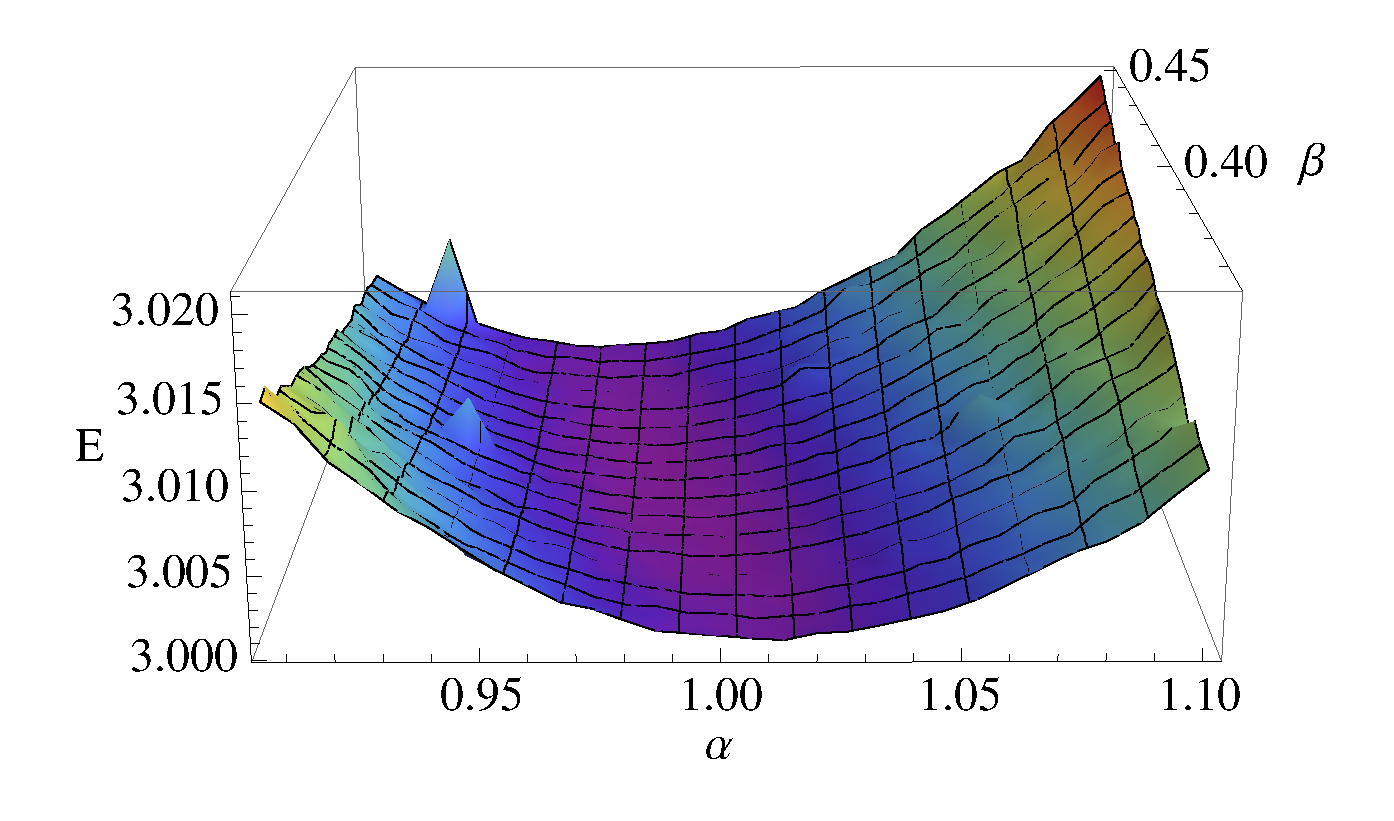
\includegraphics[scale=0.6]{2electron}
    \caption{Plot of $\alpha$- and $\beta$-dependencies of the ground state energy for two interacting electrons at the ground state based on a simulation involving 3 000 000 Metropolis cycles}
    \label{fig:2electron}
\end{figure}
\begin{figure}[htbp]
    \centering
    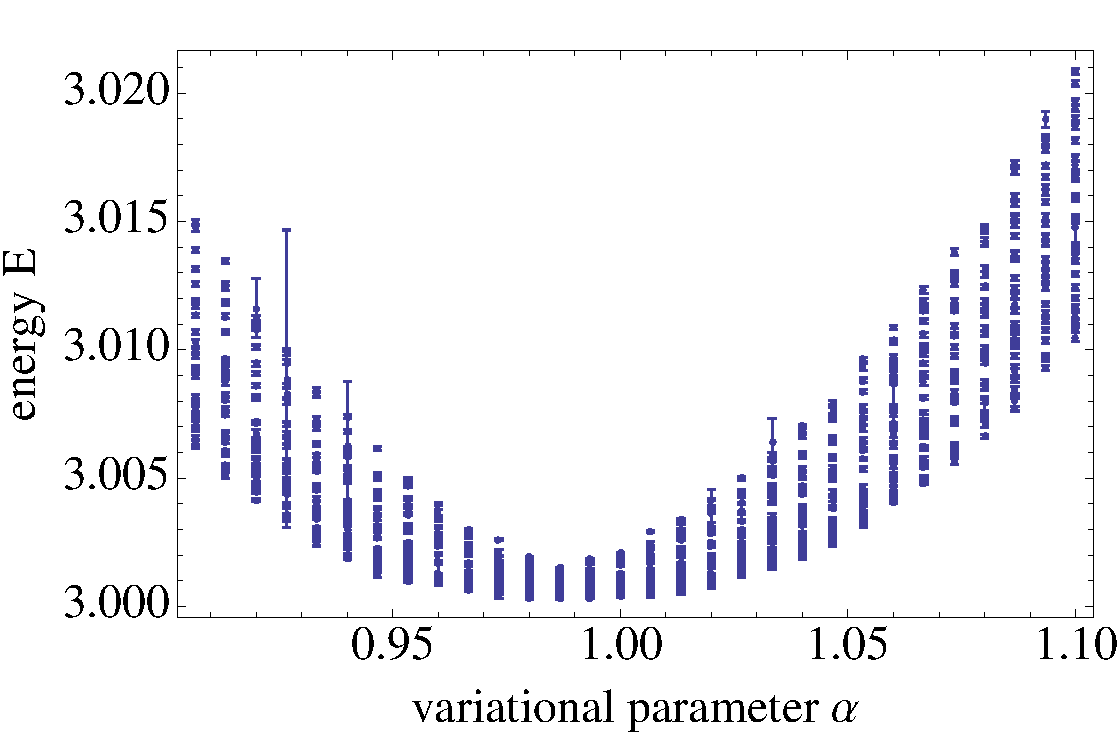
\includegraphics[scale=0.6]{2electronalpha}
    \caption{Plot of $\alpha$-dependency of the ground state energy for two interacting electrons at the ground state for different $\beta$ based on a simulation involving 3 000 000 Metropolis cycles}
    \label{fig:2electronalpha}
\end{figure}
\FloatBarrier
\subsubsection{Jastrow factor}
After computing the ground state energy we now analyse the changement in energy arising from different osciallator potentials $\omega$. The results for $\omega =\{1,0.28,0.01\}$ are shown in table~\ref{tab:omega}. It can be observed, that for small oscillator frequency the kinetic energy drops relative to the total energy of the system. The reason for this is, that for small $\omega$ the potential gets wider, but flatter as well. In this case, the electrons interact less with each other, which results in decreasing kinetic energy.\\
\begin{table}[H]
\centering
\caption{Kinetic and potential energy depending on the oscillator frequency $\omega$}
    \begin{tabular}{c|cc|c}
   \toprule
    $\omega$ & $E_{kin}$  & $E_{pot}$  & $E_{kin} (\%)$ \\ 
    \midrule
    0.01   & 0.010 & 0.064 & 14          \\
    0.28   & 0.248  & 0.773  & 24       \\
    0.50    & 0.452  & 1.206   & 27         \\
    0.70    & 0.607  & 1.600   & 28           \\
    1.00      & 0.862  & 2.137   & 29          \\
    \bottomrule
    \end{tabular}
\label{tab:omega}
\end{table}
In the wave equation
\begin{equation}
\psi_T(\mathbf{r_1,r_2}) = C \exp\left[-\alpha\frac{\omega}{2} (r_1^2+r_2^2)\right] \exp \left[ \frac{a_{12} r_{12}}{(1+\beta r_{12})} \right]
\end{equation}
only the first exponential term is affected by the oscillator frequency $\omega$, while the Jastro factor does not contain the frequency.\\
For vanishing potential as for $\omega =0.01$ the wave function becomes:
\begin{equation}
\lim_{\omega\rightarrow 0} \psi_T(\mathbf{r_1,r_2}) = C \exp \left[ \frac{a_{12} r_{12}}{(1+\beta r_{12})} \right] = C J,
\end{equation}
where $J$ is the Jastrow factor. This means, that in this case the Jastrow factor adopts a more important role. The correlations introduced by the Jastro factor \todo{correlations of Jastro factor}
\subsubsection{Importance sampling: $\delta t$-dependency}
To obtain accurate results we also introduce important sampling and optimize the calculation of the energy by studying its time step dependency. We will refer to the time step as $\delta t$. The time step plays an important role in importance sampling, since it the biasing when calculation new random numbers. For large $\delta t$ the newly picked random numbers for the particle position can vary more, than for smaller $\delta t$. It is therefore relevant to use a reasonable time step to aviod jumping to far in the position or to get stuck in one place as explained previously in section~\ref{sec:importance}. In figure~\ref{fig:importance} we plotted the energy calculated for $\alpha = 0.98$ and $\beta = 0.40$ (according to~\ref{sec:2electron}) for diverse $\delta t$. Comparing the results including importance sampling to those in section~\ref{sec:2electron} we notice, that with importance sampling we can obtain a lot smaller energies, than when using a brute force Metropolis algorithm. This shows, that the importance sampling has an impact on the precision of the results, because we get energies very near the exact solution.\\
Concerning the optimal value of $\delta t$, it is obvious in figure~\ref{fig:importance}, that it must be $\delta t \in [0.1,0.2]$. Because of the statistical spread of the energy values, we cannot find the one and only perfect $\delta t$-value. For large time steps, that are still smaller than $\delta t= 4$ the energy converges to $E=3.002$. For even higher time steps, the calculated energy increases strongly and precise simulations become impossible.
\begin{figure}[htbp]
    \centering
    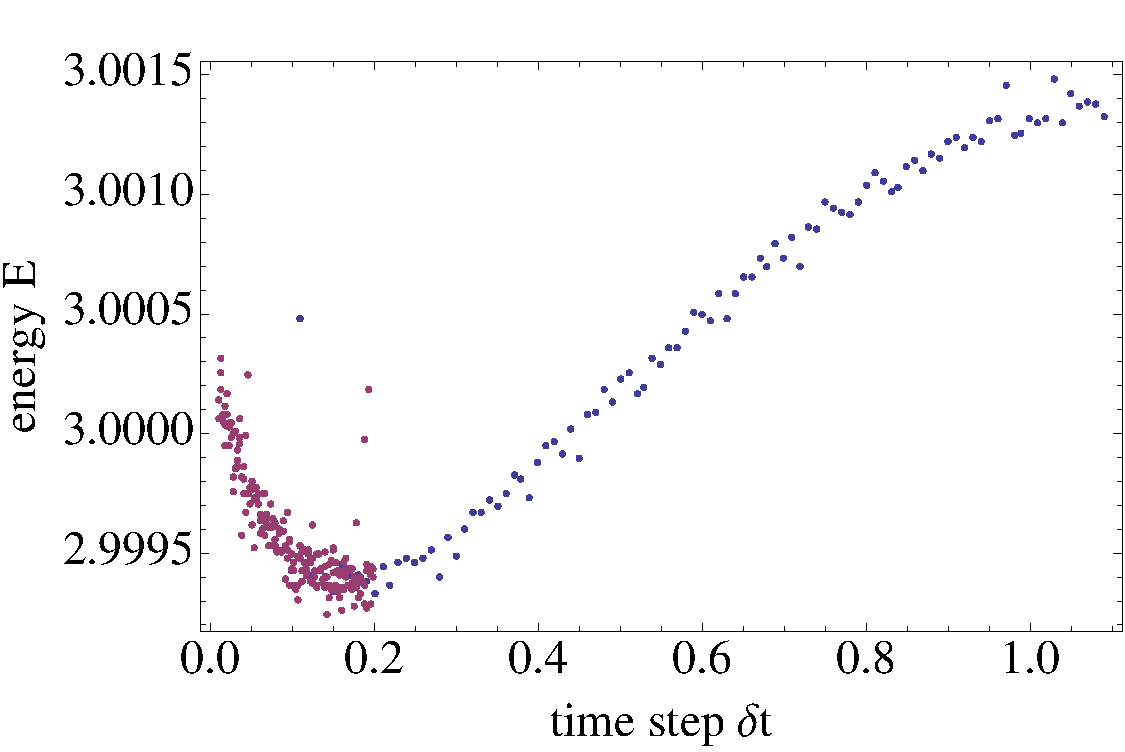
\includegraphics[scale=0.6]{importance}
    \caption{Results of energy calculation for varying time steps $\delta t$ in the importance sampling. The blue dots refer to a wide-spaced simulation for $\delta t \in [0.1,1]$ with step length $\Delta (\delta t) = 0.01$, whereas the violet dots refer to $\delta t\in [0.01,0.2]$ with $\Delta(\delta t) = 0.001$}
    \label{fig:importance}
\end{figure}
\FloatBarrier

\subsection{Six electron case}
In this part we introduce the six electron case. In order to do so we consider the more general trial wave function \ref{glg:6electron} which also includes the case of two electrons. The simulations are done like in section \ref{sec:2electron} but with $400000$ cycles, because of higher computation times.

\subsubsection{Perturbed Case}\label{sec:perturbed_six}
For the perturbed six electron system the ground state energies are shown in table \ref{tab:groundstate_sixelectron}. Comparing the energies with \citet[TABLE III]{lohne2011} we have a good agreement but slightly larger values. For increasing $\omega$ we have higher values of $\alpha$ and $\beta$. Figure \ref{fig:alpha_beta_omega} shows the dependencies in this case. It can be seen that there is no easy linear coherence, instead we made an arbitrarily chosen fit with a square-root function which seemed for us the best approximation and deals a reference where to search for the energy minima for different $\omega$. 
\begin{table}
    \centering
    \caption{Ground state energies for six electrons in an oscillator well.}
    \begin{tabular}{c|cc|c}
    $\omega$   & $\alpha$    & $\beta$ &    $E$    \\ \hline
    $1.00$     & $0.98$      & $0.45$  & $20.185$  \\
    $0.5$      & $0.925$	    & $0.38$  & $11.8047$ \\
    $0.28$     & $0.8$       & $0.25$  & $7.736$   \\
    $0.01$     & $0.7$       & $0.08$  & $0.6986$  \\
    \end{tabular}
    \label{tab:groundstate_sixelectron}
\end{table}
\begin{figure}[htbp]
    \centering
    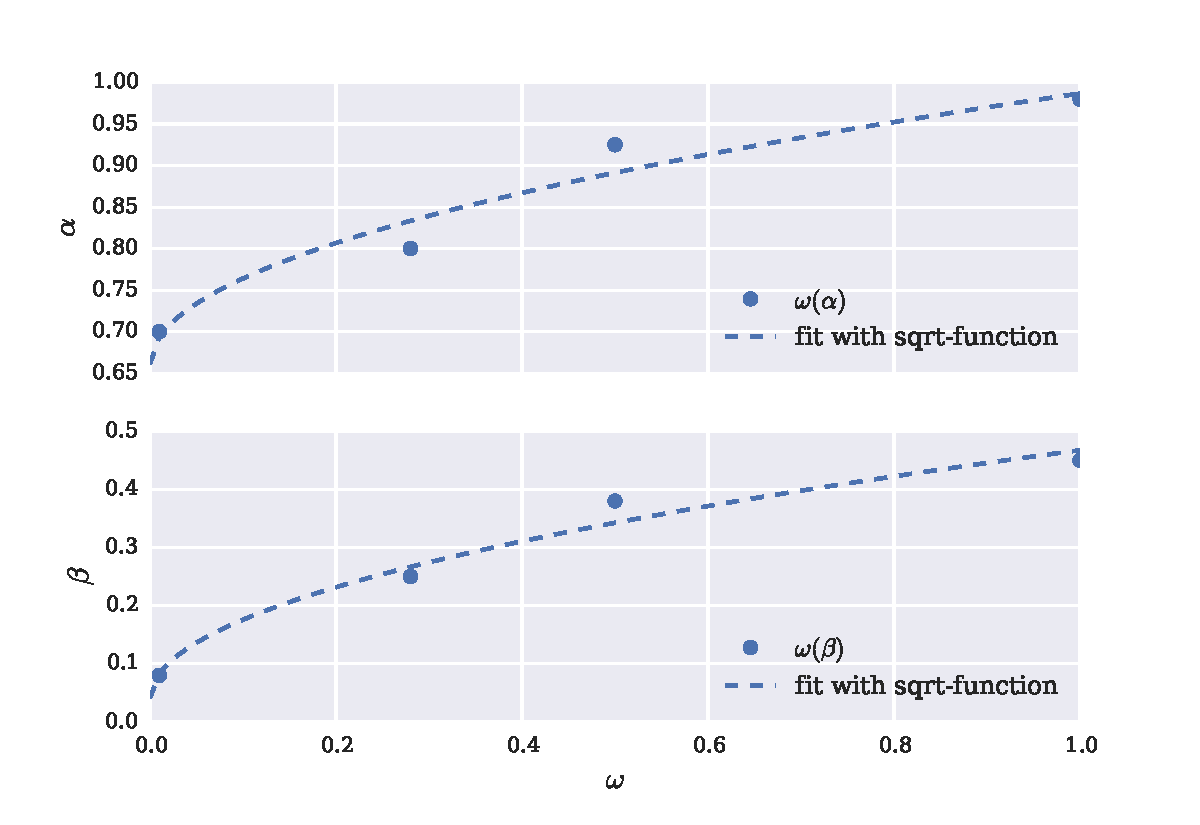
\includegraphics[scale=0.7]{alpha_beta_omega.pdf}
    \caption{Shows the dependency between the locations of the energy minima and the variational parameter.}
    \label{fig:alpha_beta_omega}
\end{figure}

All in all our code seems to calculate reliable and good energies. Nevertheless we had to struggle with rather seldom but randomly appearing negative kinetic energies in single cores when using importance sampling. Changing our initial guesses for the starting positions increased here the quality of the solution considerably. In Appendix \todo{reference} are shown some three-dimensional plots which show the problem. 

\subsubsection{Unperturbed Case}
We know that with switched off electron-electron repulsion the lowest energy value should become $10\,\omega$, since we are observing six electrons. In figure \ref{fig:six_electron_unperturbed} this relation is shown for different $\omega$ over $\alpha$ and it can be observed that our results fit very well to the theory. 
\begin{figure}[htbp]
    \centering
    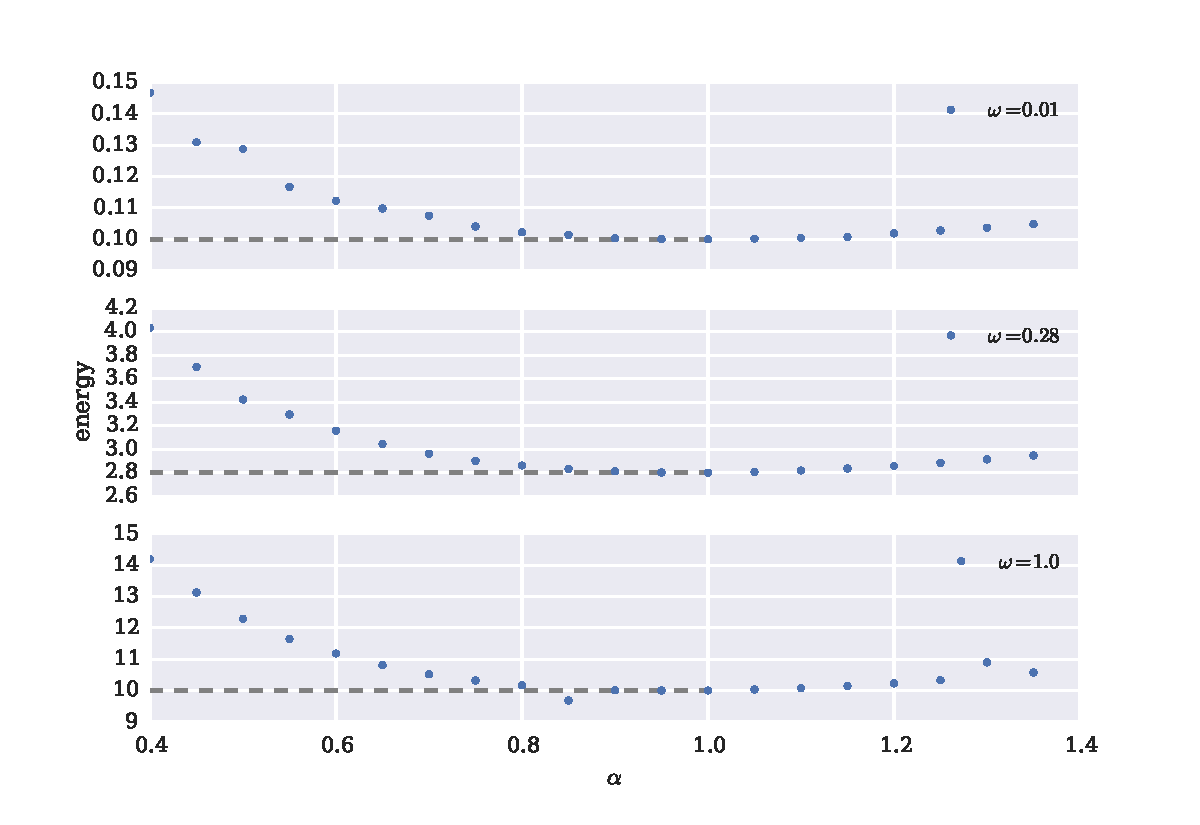
\includegraphics[scale=0.7]{six_electron_unperturbed}
    \caption{The figure shows the energy plotted over the variational parameter $alpha$ assuming six electrons without the repulsive electron-electron forces. For different values of $\omega$ the minimum lies at $10\omega$ which is coherent with the theoretical view.}
    \label{fig:six_electron_unperturbed}
\end{figure}

\subsubsection{Virial theorem}
The virial theorem states a relationship between the mean of the potential $\langle V \rangle$ and of the kinetic energy $\langle T \rangle$ of a closed system. This is described by
\begin{equation}
    \gamma \langle V \rangle = 2 \langle T \rangle,
\end{equation}
with $\gamma$ the homogeneity of the potential $V$. This means for a harmonic oscillator which potential goes with the power of $2$ that one can expect the relationship $\langle V \rangle = \langle T \rangle$. However if we consider the perturbed wavefunction we have additional terms which are stated by the repulsion of the electron and would reveal $\gamma = -1$. Hence, we can make the prediction that the perturbed wavefunction should yield to a smaller ratio 
\begin{equation}
\left(\frac{\langle V \rangle}{\langle T \rangle}\right)_{perturbed} \leq \left(\frac{\langle V \rangle}{\langle T \rangle}\right)_{unperturbed},
\end{equation}
whereas the difference should be larger for smaller $\omega$, because thereby the oscillator potential becomes less relevant. Meanwhile for different $\omega$ and the unperturbed case the ratio should not change and be unity.

In figure \ref{fig:virialtheorem} this behaviour is shown and mostly consistent. Considering first the two electron case we can observe for the unperturbed wavefunction a ratio that is nearly one for all omega. The perturbed part indeed shows the predicted behaviour that it is firstly smaller and secondly it increases with increasing omega. For the six electron system the perturbed functions have the same dependencies as for two electrons with even smaller ratios. This can be physically understood as a more important role for the electron-electron interactions in the six electron case which go with $\gamma = -1$. For the unperturbed part there is a small deviation to unity for larger omegas. This shouldn't be the case and reveals a potential problem in the code for multiple particles. Indeed the data shows that there might be an issue in the draft of the slater matrix. However taking also in reference the known issues of section \ref{sec:perturbed_six} it could also depend on the important sampling but still after extensive search we were not able to find a malfunction and all other calculations run reasonable which leads us to the conclusion that the energies that are produced by our code are reliable values.  
\begin{figure}[htbp]
    \centering
    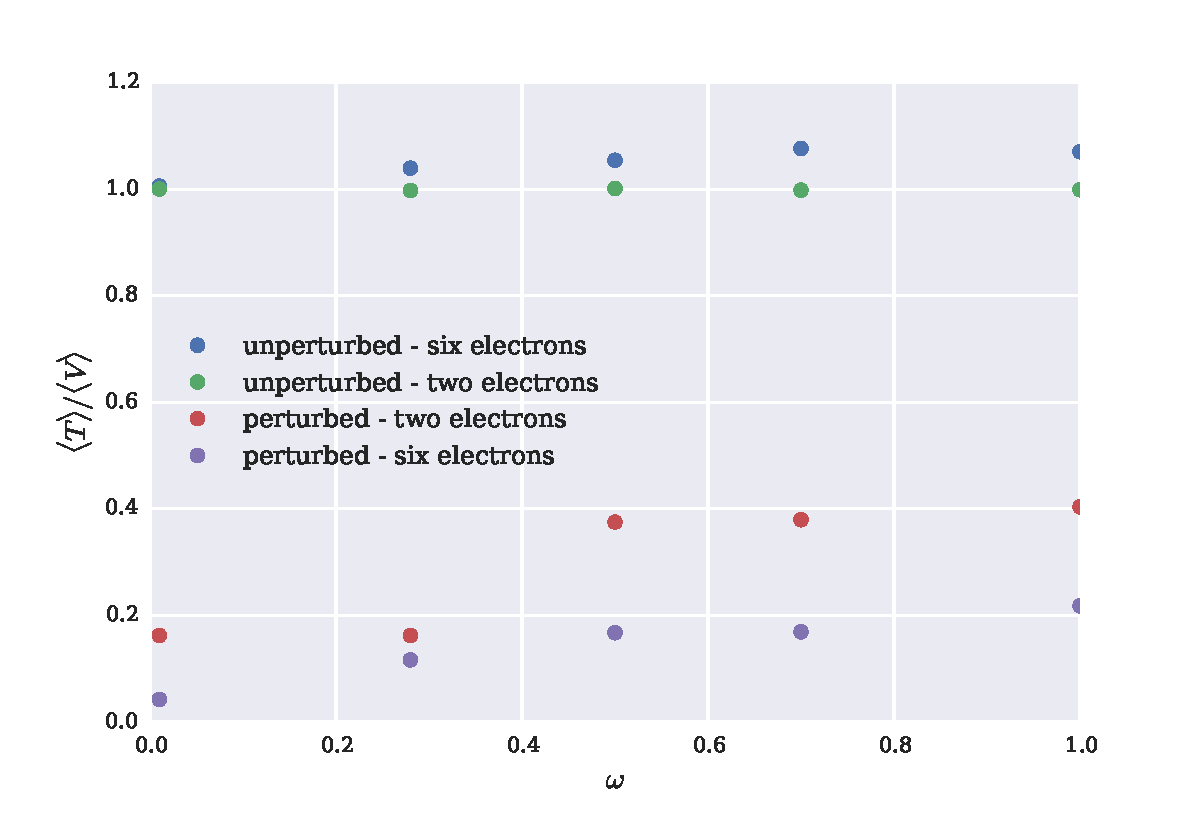
\includegraphics[scale=0.7]{virialtheorem}
    \caption{Shows the fraction of the mean kin. energy $\langle T \rangle$ to the mean pot. energy $\langle V \rangle$ for different values of $\omega$. The calculations are done with either two or six electrons. The unperturbed function}
    \label{fig:virialtheorem}
\end{figure}

\subsection{Closed form solutions}\label{sec:analytical}
Finally we still want to introduce calculations with the closed form solutions described in section \ref{sec:closed_form}. For that reason the program was restructured in parts and new classes for the Jastrow-factor and the Slater-matrix were introduced. This can be found at the separate branch \texttt{closed_form} at the provided git repository. The part is fully implemented but unfortunately we were not able to reproduce the solution of the brute force approximations. But still because we implemented the full code, we were able to calculate the profiling and can make first estimations how much faster the code could be. We thereby implemented no optimizations, like an improved calculation of the inverse slater matrix yet (see \citet{hogberget2013} for more details). An overview for the profiling is given in the table \ref{}\todo{reference}.
%	\include{5-Discussion}
	\section{Conclusion}\label{sec:conclusion}
In this project, we have preformed a Variational Monte Carlo simulation computing the energies of various electron systems.

In good accordance to~\cite{hogberget2013} we have calculated the ground state energy of two electrons in a (harmonic oscillator) trap at $E=3.0003$ as well as for diverse oscialltor frequencies. Introducing importance sampling we have analysed the importance of the time step $\delta t$ in the sampling noticing, that the simulation is stable for a range of $\delta t < 3$. Moving on to six electrons it turned out, that the time step is responsible for the simulation stability. For inappropriate $\delta t$ we experienced outliers in the energy calculation, that can be seen in figure~\ref{fig:psix1} and~\ref{fig:psix05}. Overall the calculated energies correspond pretty well to those found by~\cite{hogberget2013} and~\cite{lohne2011}, which indicates that although those problems continue existing, we were able to extract suitable output from the simulation.

Another evidence, that the calculations are correct is given by the fact, that the virial-theorem is confirmed by our computations apart from small errors.

Furthermore, we were able to propose a relation of the variational parameters and the oscillator frequency in section~\ref{sec:perturbed_six}. 

In order to show the advantages of closed-form solutions towards brute-force derivations we compared the time profile. Here it showed off that especially for larger electron systems the closed-form can deliver more performant calculations.  
	\begin{appendix}
\section{3D Plots}
We will now show the energy's dependencies on the variational parameters $\alpha$ and $\beta$ first for the case of two interacting electrons and then for the case of six interacting electrons in a harmonic oscillator potential.
\subsection{Two electron perturbed case}
\begin{SCfigure}[30][h]
    \centering
    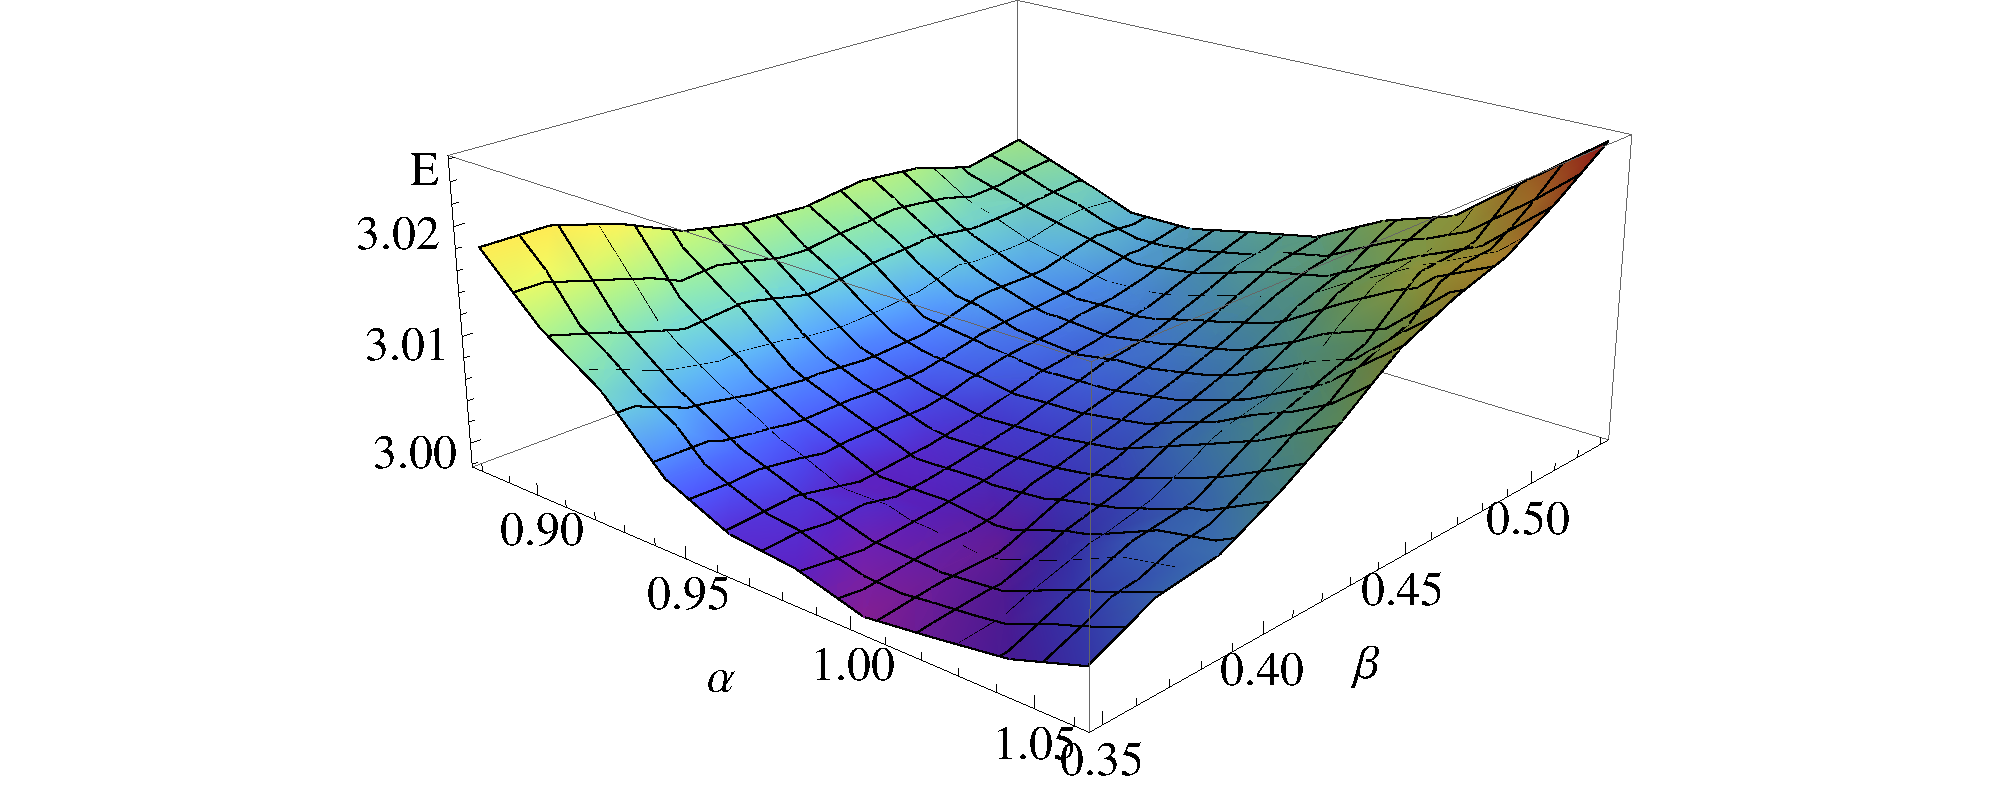
\includegraphics[scale=0.36]{ptwo1}
    \caption{Plot of $\alpha$- and $\beta$-dependencies of the ground state energy for two interacting electrons at the harmonic oscillator frequency $\omega=1$}
    \label{fig:ptwo1}
\end{SCfigure}
\begin{SCfigure}[30][h]
    \centering
    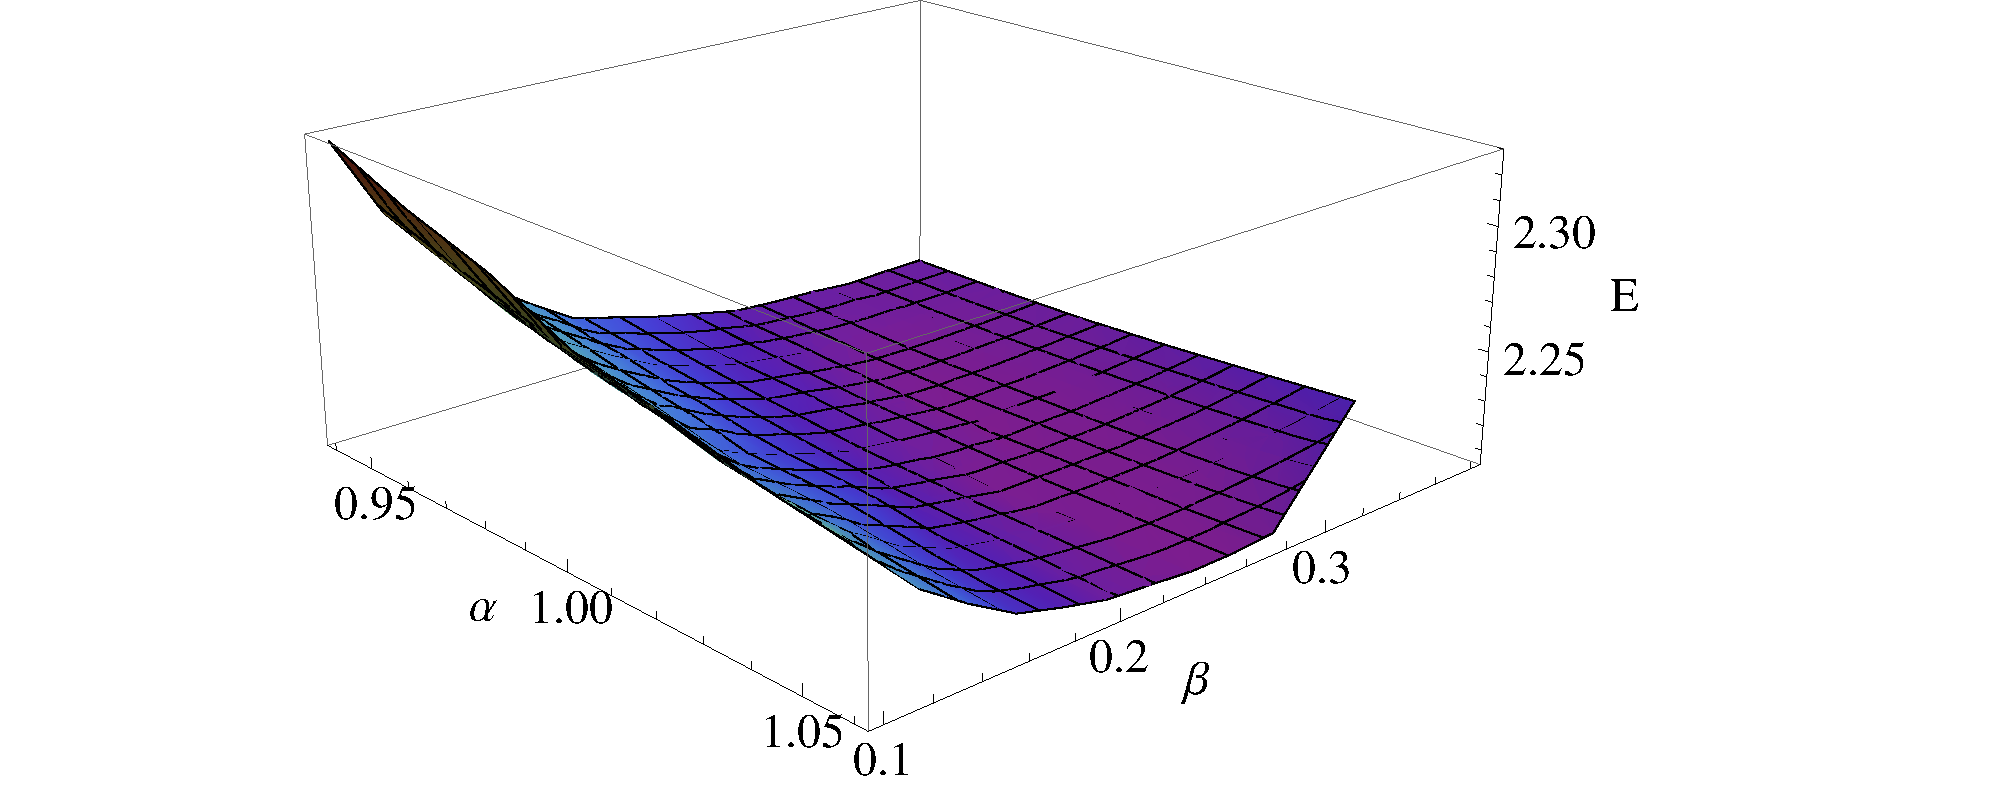
\includegraphics[scale=0.36]{ptwo07}
    \caption{Plot of $\alpha$- and $\beta$-dependencies of the ground state energy for two interacting electrons at the harmonic oscillator frequency $\omega=0.7$}
    \label{fig:ptwo07}
\end{SCfigure}
\begin{SCfigure}[30][h]
    \centering
    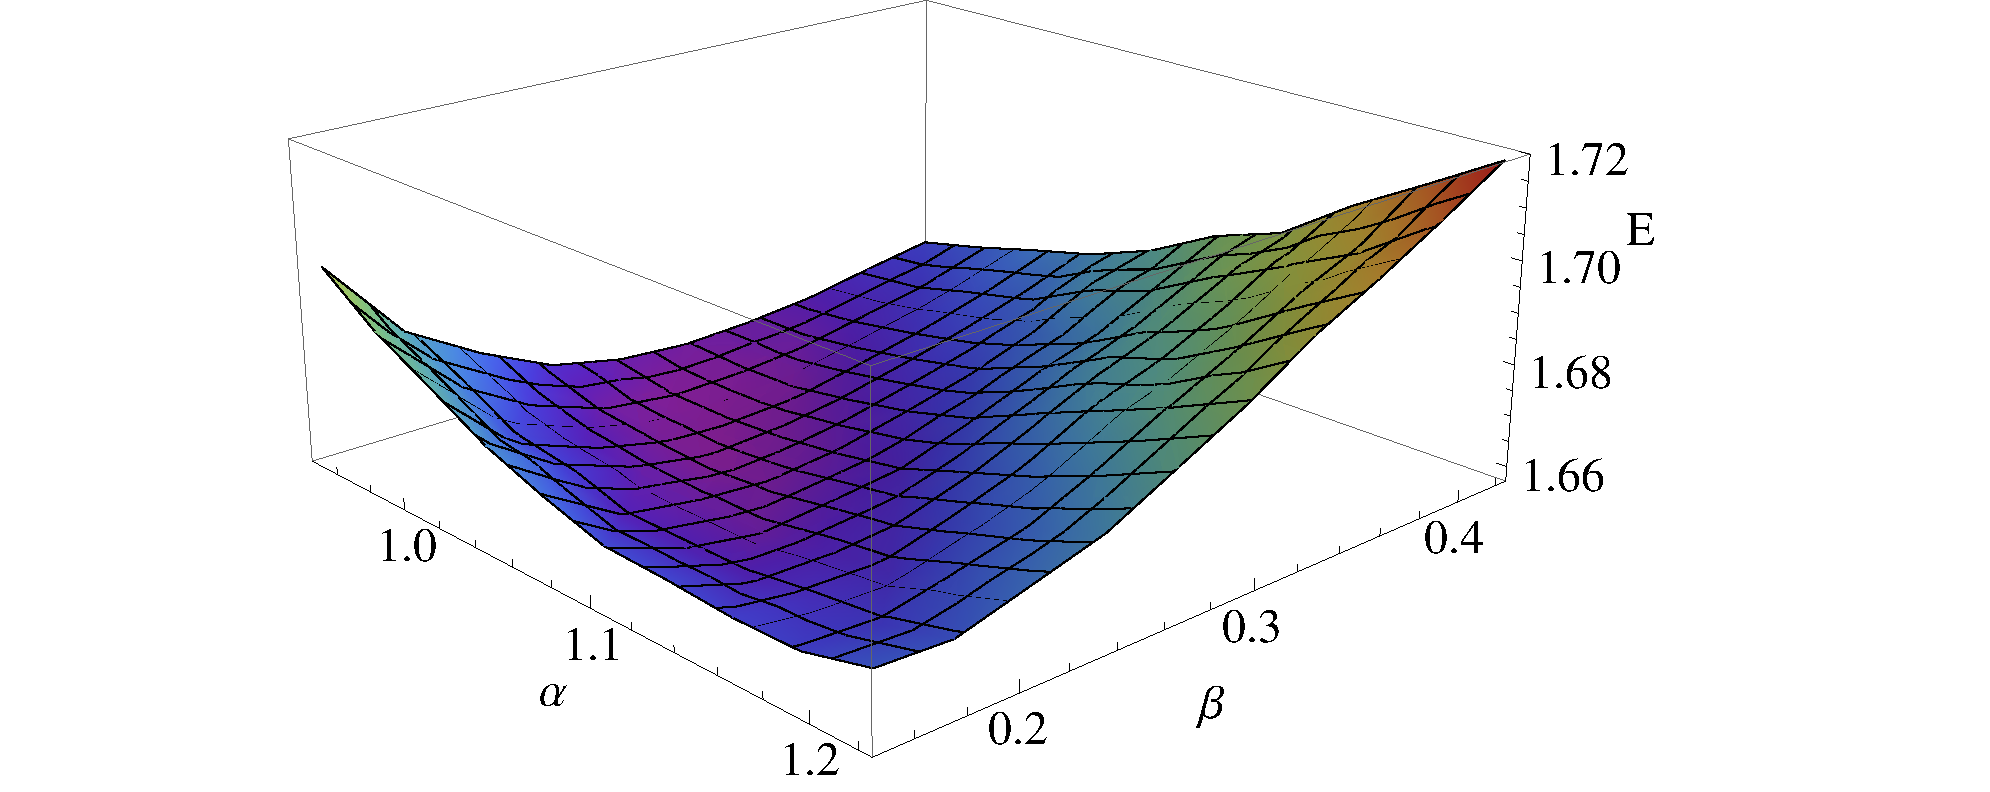
\includegraphics[scale=0.36]{ptwo05}
    \caption{Plot of $\alpha$- and $\beta$-dependencies of the ground state energy for two interacting electrons at the harmonic oscillator frequency $\omega=0.5$}
    \label{fig:ptwo05}
\end{SCfigure}
\begin{SCfigure}[30][h]
    \centering
    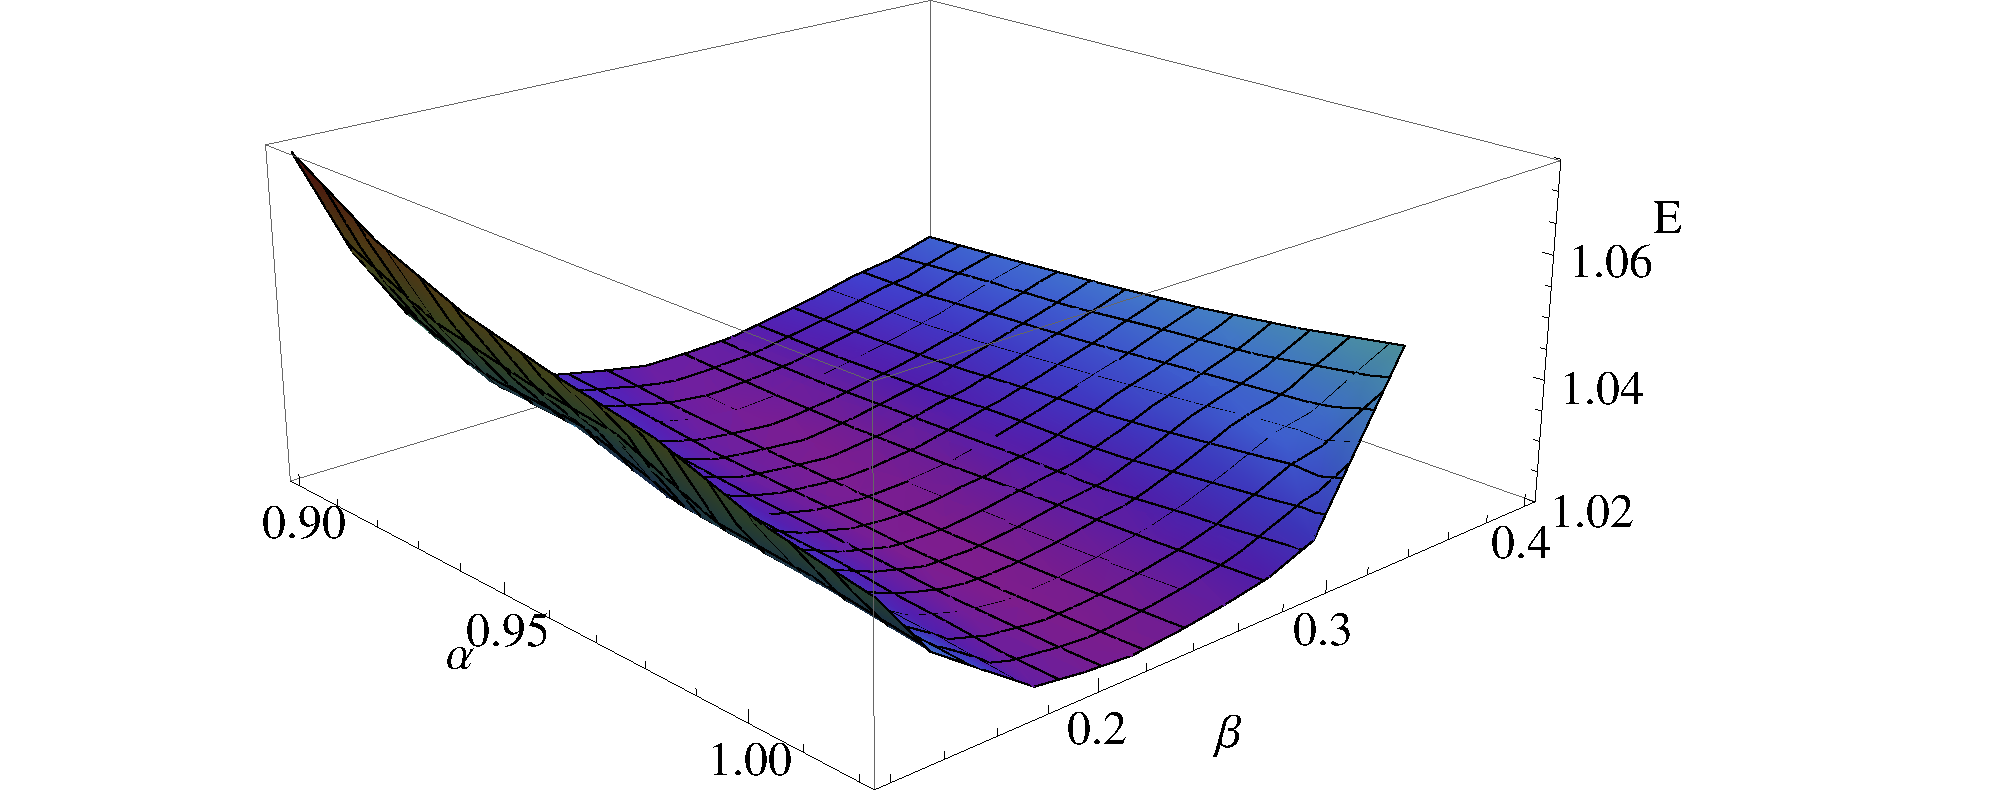
\includegraphics[scale=0.36]{ptwo028}
    \caption{Plot of $\alpha$- and $\beta$-dependencies of the ground state energy for two interacting electrons at the harmonic oscillator frequency $\omega=0.28$}
    \label{fig:ptwo028}
\end{SCfigure}
\begin{SCfigure}[30][h]
    \centering
    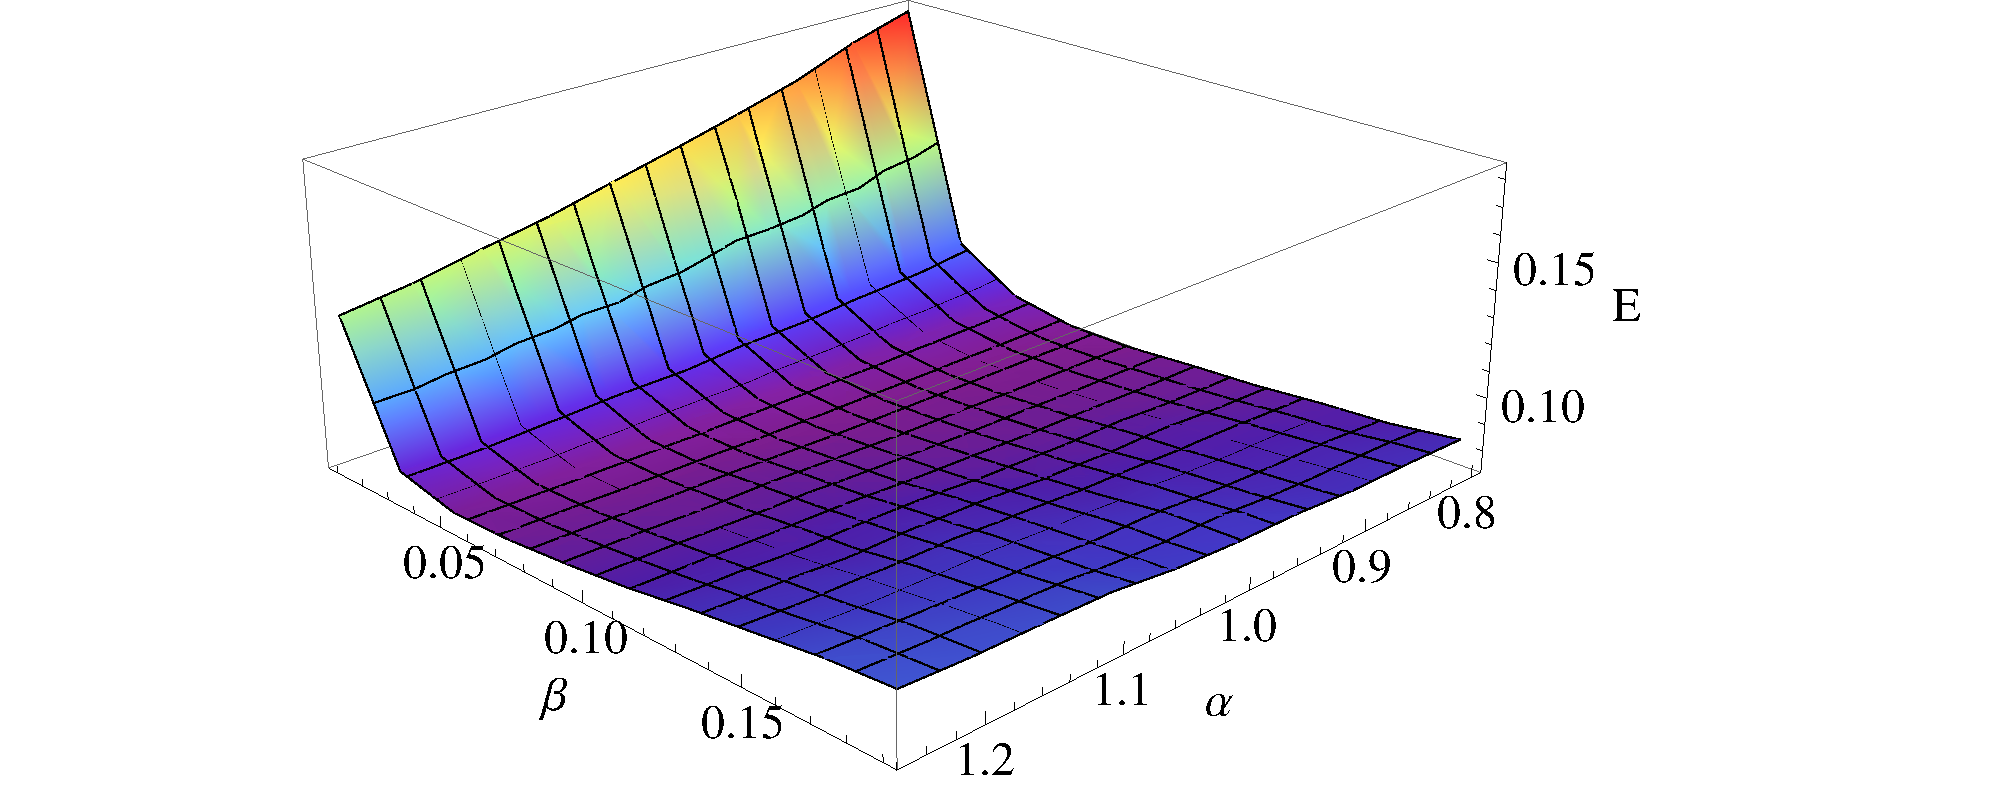
\includegraphics[scale=0.36]{ptwo001}
    \caption{Plot of $\alpha$- and $\beta$-dependencies of the ground state energy for two interacting electrons at the harmonic oscillator frequency $\omega=0.01$}
    \label{fig:ptwo001}
\end{SCfigure}
\FloatBarrier
\subsection{Six electron perturbed case}\label{sec:app_six_electron}
\begin{SCfigure}[30][h]
    \centering
    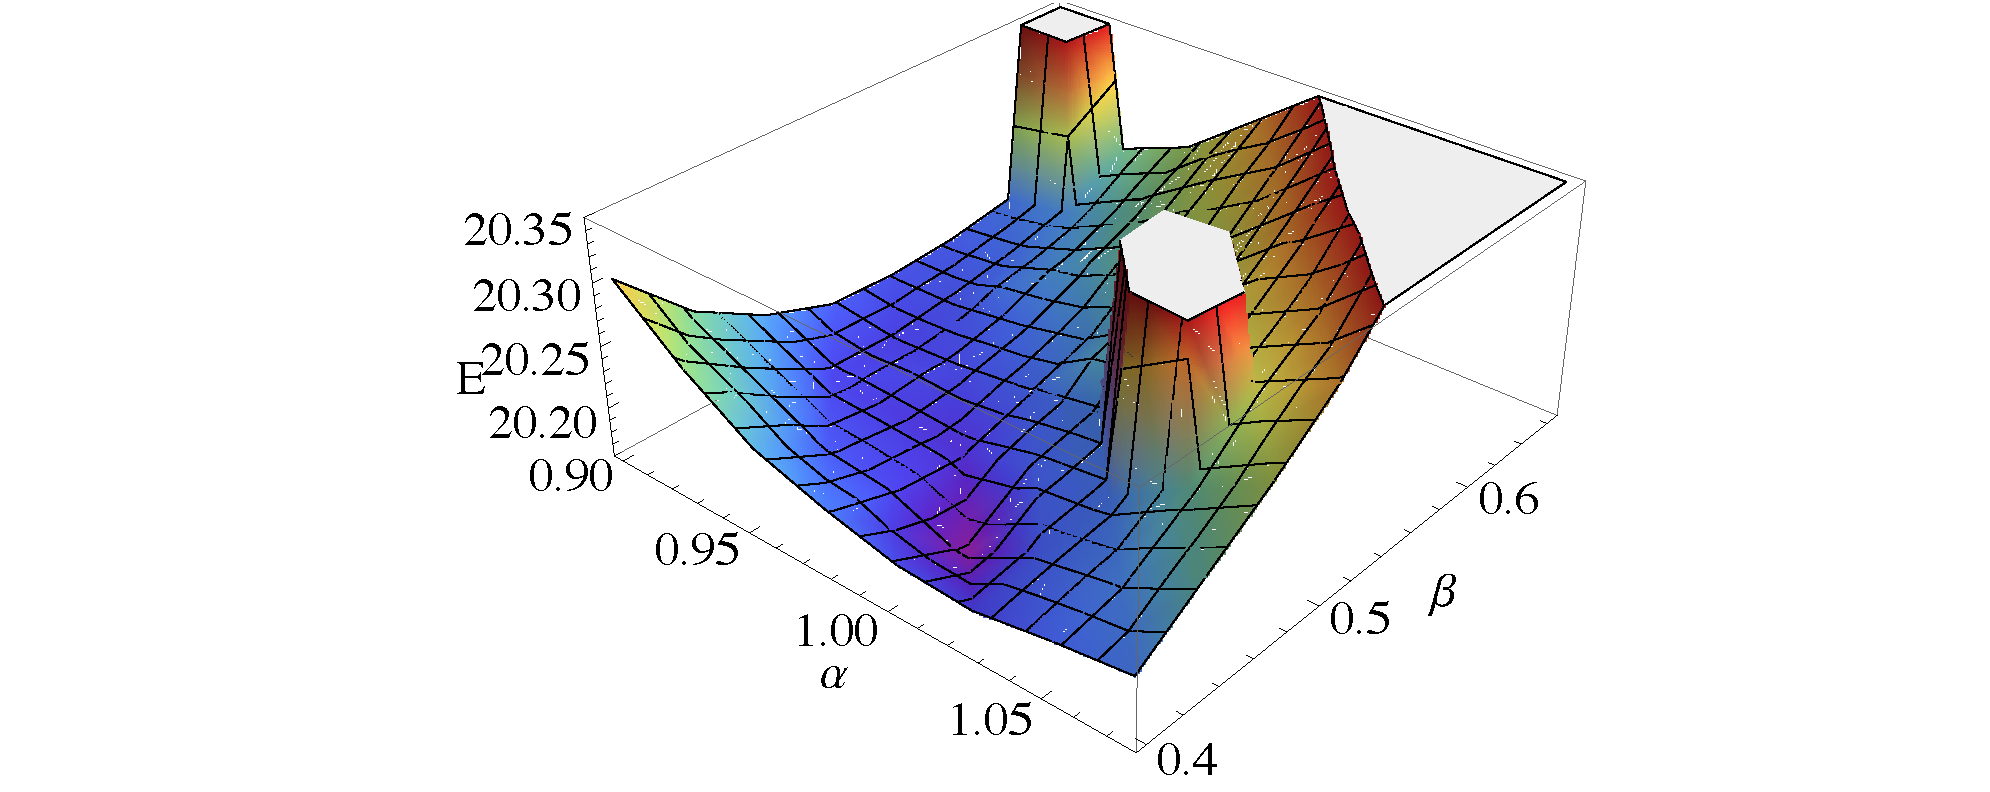
\includegraphics[scale=0.48]{psix1}
    \caption{Plot of $\alpha$- and $\beta$-dependencies of the ground state energy for six interacting electrons at the harmonic oscillator frequency $\omega=1$}
    \label{fig:psix1}
\end{SCfigure}
\begin{SCfigure}[25][h]
    \centering
    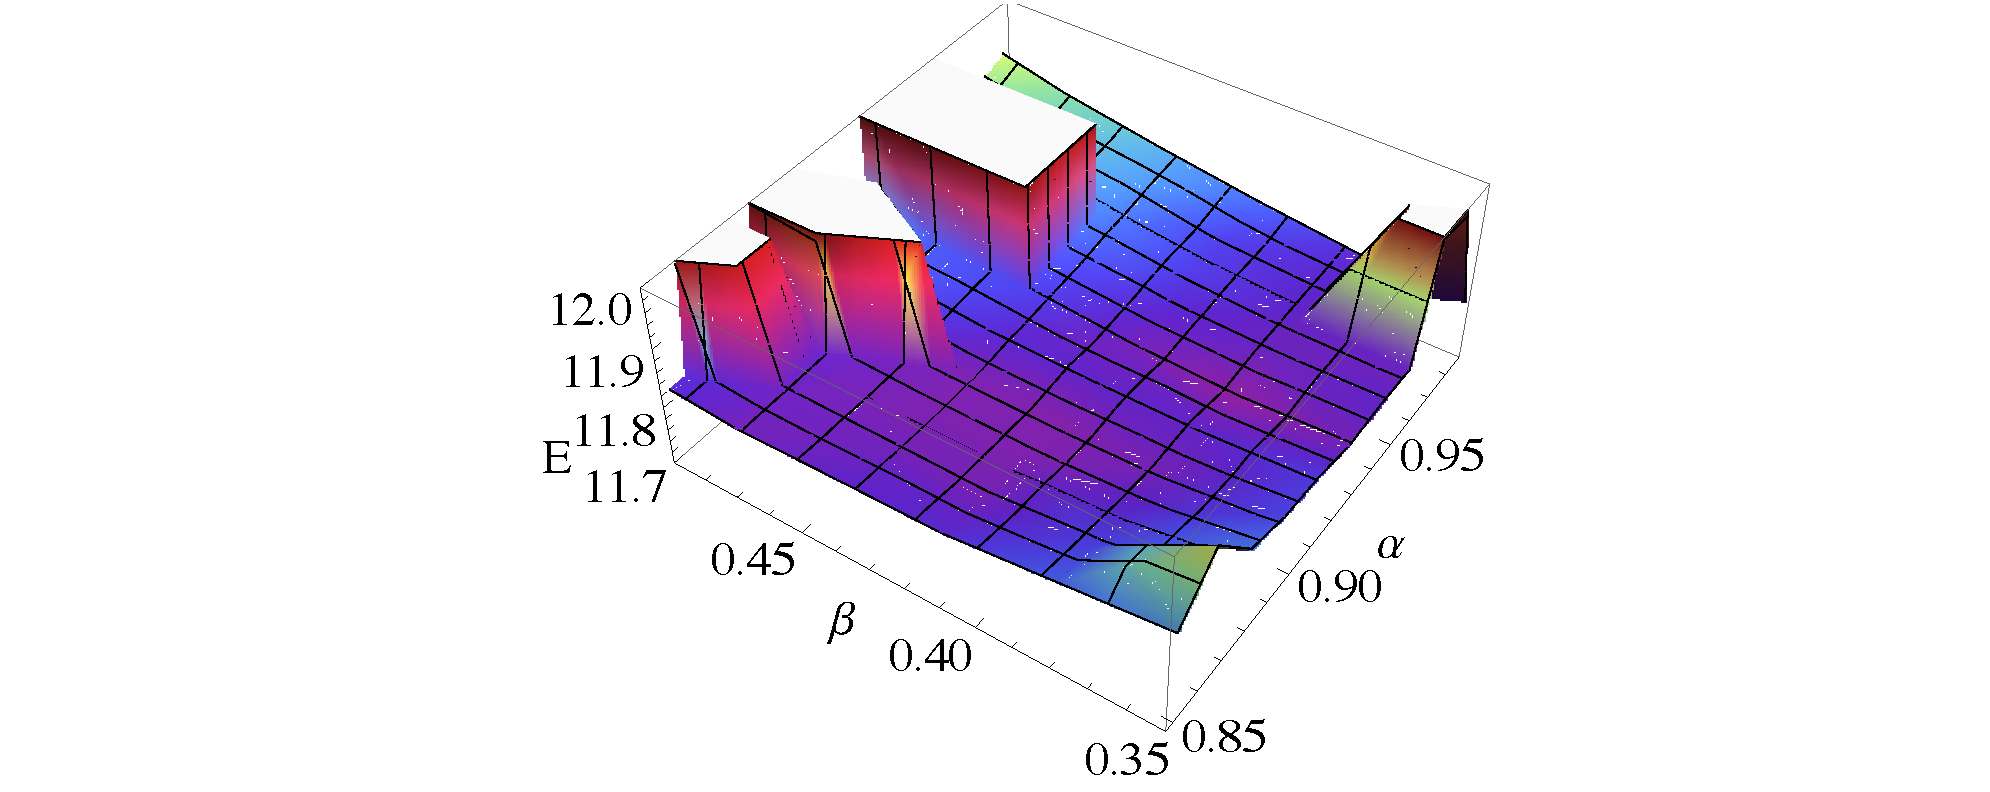
\includegraphics[scale=0.53]{psix05}
    \caption{Plot of $\alpha$- and $\beta$-dependencies of the ground state energy for six interacting electrons at the harmonic oscillator frequency $\omega=0.5$}
    \label{fig:psix05}
\end{SCfigure}
\begin{SCfigure}[30][h]
    \centering
    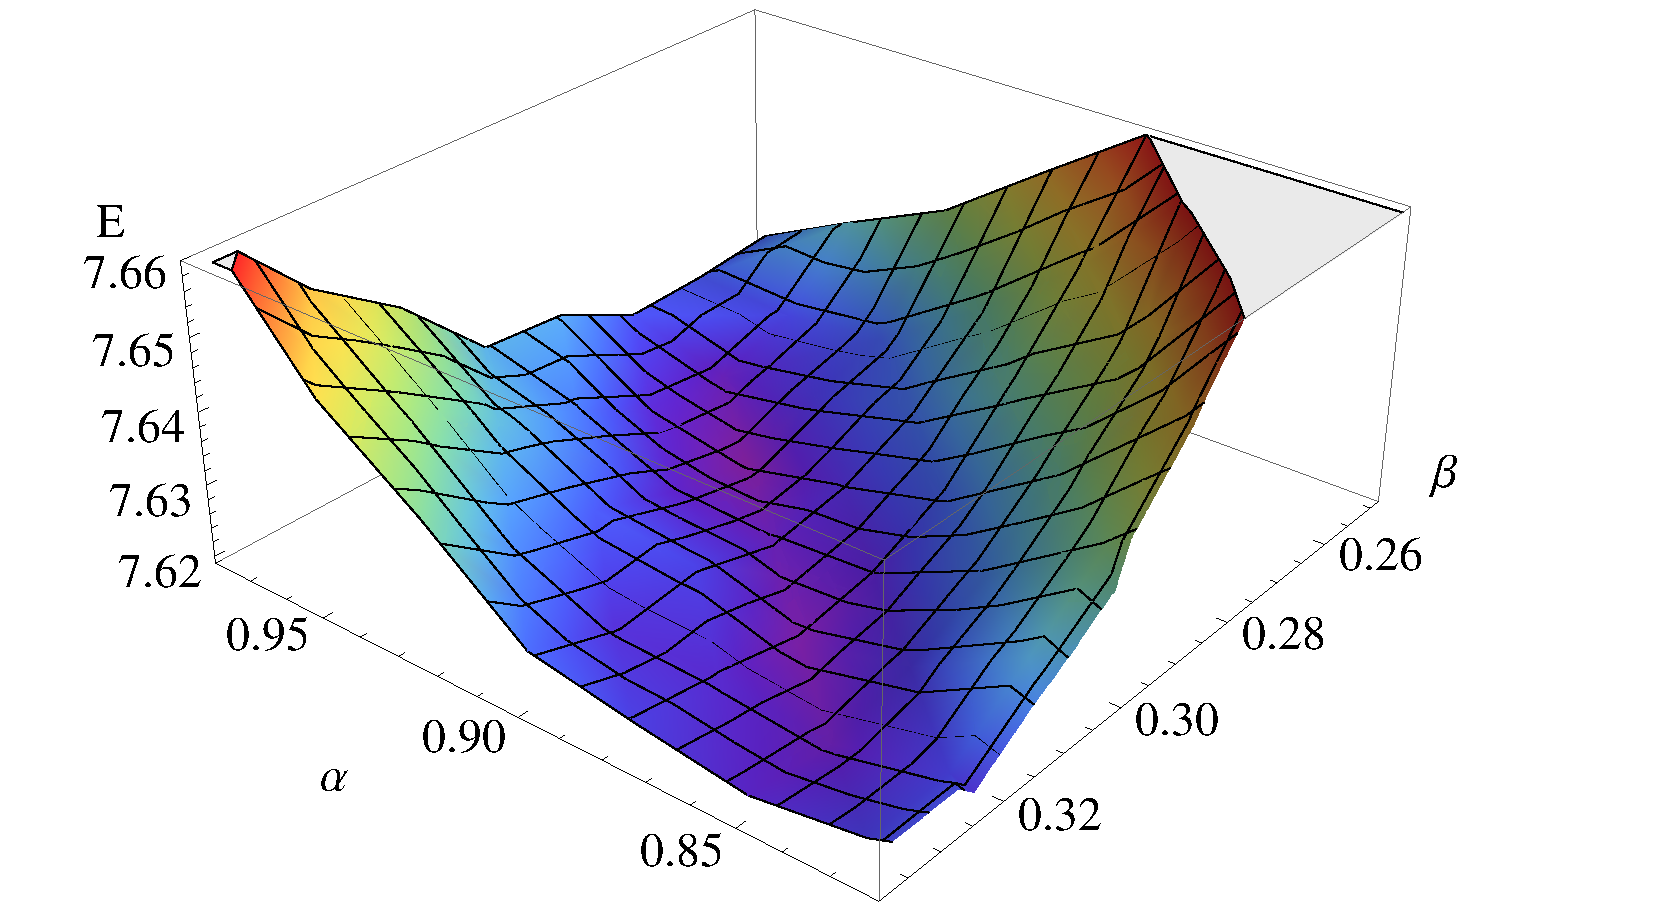
\includegraphics[scale=0.35]{psix028}
    \caption{Plot of $\alpha$- and $\beta$-dependencies of the ground state energy for six interacting electrons at the harmonic oscillator frequency $\omega=0.28$}
    \label{fig:psix028}
\end{SCfigure}
\begin{SCfigure}[30][h]
    \centering
    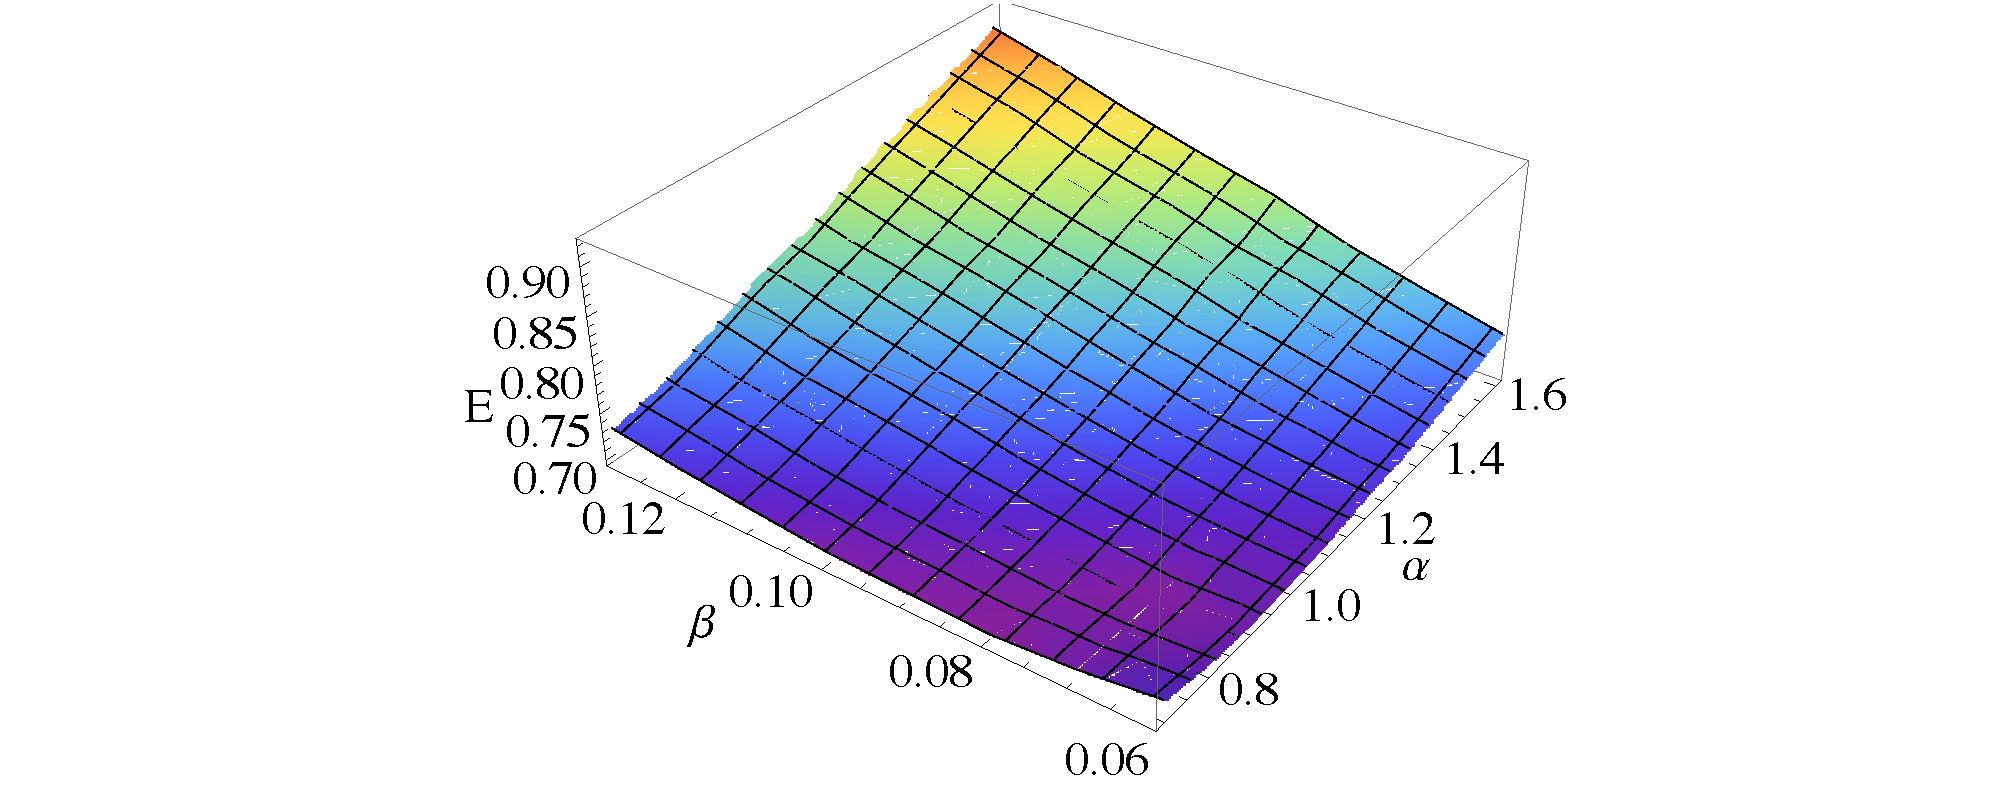
\includegraphics[scale=0.5]{psix001}
    \caption{Plot of $\alpha$- and $\beta$-dependencies of the ground state energy for six interacting electrons at the harmonic oscillator frequency $\omega=0.01$}
    \label{fig:psix001}
\end{SCfigure}
\end{appendix}   
        \bibliography{Literatur}
\end{document}